%%%%%%%%%%%%%%%%%%%%%%%%%%%%%%%%%%%%%%%%%
% Medium Length Professional CV
% LaTeX Template
% Version 2.0 (8/5/13)
%
% This template has been downloaded from:
% http://www.LaTeXTemplates.com
%
% Original author:
% Trey Hunner (http://www.treyhunner.com/)
%
% Important note:
% This template requires the resume.cls file to be in the same directory as the
% .tex file. The resume.cls file provides the resume style used for structuring the
% document.
%
%%%%%%%%%%%%%%%%%%%%%%%%%%%%%%%%%%%%%%%%%

%----------------------------------------------------------------------------------------
%	PACKAGES AND OTHER DOCUMENT CONFIGURATIONS
%----------------------------------------------------------------------------------------

\documentclass{resume} % Use the custom resume.cls style

\usepackage[hmargin={2.5cm,2.0cm}, vmargin={2.1cm,2cm}]{geometry} % Document margins
\usepackage[pdftex,colorlinks=true,urlcolor=blue]{hyperref}
\usepackage[english,printdayoff]{isodate}
\usepackage{tabularx}
\usepackage[T1]{fontenc}
\usepackage[utf8]{inputenc}
\usepackage[english]{babel}
\usepackage{graphicx}

\newcommand{\myemail}{andrey.rjeutski@outlook.com}
\newcommand{\minsk}{Minsk, Belarus}

\begin{document}

\begin{rHeader}{
\printname{Andrey Rjeutski}
\printaddress{+49 1575 7742255 \\ \href{mailto:\myemail}{\myemail}}
\printaddress{Eligible to work in Germany for any employer}
\printaddress{Occamstraße 21 \\ 80802 Munich}
}
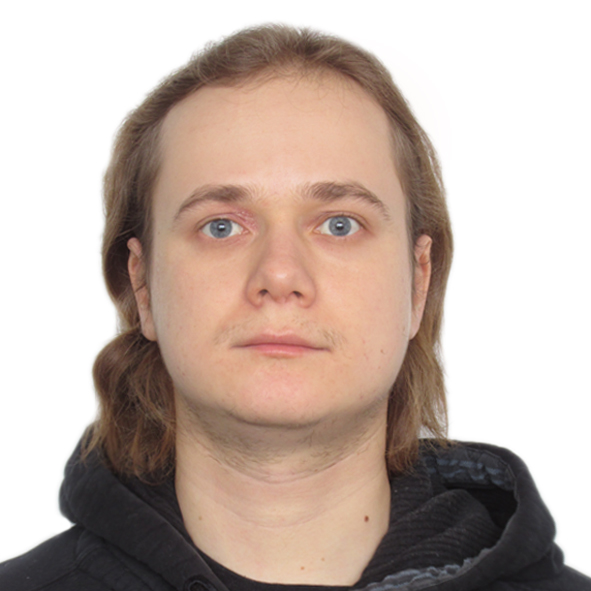
\includegraphics[width=0.95\textwidth]{photo.jpg}
\end{rHeader}

%----------------------------------------------------------------------------------------
%	WORK EXPERIENCE SECTION
%----------------------------------------------------------------------------------------

\begin{rSection}{Experience}

\begin{rSubsection}
{\href{https://www.brainloop.com}{Brainloop AG}}
{\printdate{2016-04-01} to present}
{Software Engineer}
{Munich, Germany}
\item Developed a cross-platform Dropbox-like file management application for different
mobile and desktop systems (Android, iOS, Windows and Windows Store).
\item Implemented Microsoft Outlook add-in for an enterprise file sync and share 
service.
\item Improved development workflow by introducing code review process, migrating code 
from TFVC to Git and setting up continuous automated UI testing.
\item Solution stack:
  .NET,
  C\#, 
  Git,
  MEF,
  MSTest,
  NUnit,
  Ranorex,
  Sqlite,
  TFS,
  WPF,
  Xamarin.
\end{rSubsection}

%------------------------------------------------


\begin{rSubsection}
{\href{http://www.issoft.by/}{ISsoft}}
{\daterange{2012-01-01}{2015-05-01}}
{Software Engineer}
{\minsk}
\item Developed Microsoft Word add-ins for legal and life sciences industries. 
Completely rebuilt the user interface of the application and made it fast,
responsive and modern looking.
\item Implemented the test harness. Time to stabilize a release was reduced from six to 
two weeks.
\item Built a desktop application for corporate bonds interest calculation.
\item Programmed a SaaS solution to manage and monitor backups online.
\item Managed a team of five developers in team leader's absence, mentored junior team 
members.
\item Solution stack:
  .NET,
  ASP.NET MVC,
  Autofac,
  Bootstrap,
  C\#, 
  Entity Framework,
  JavaScript,
  Knockout,
  MSSQL,
  MSTest,
  Microsoft Enterprise Library,
  NUnit,
  OpenXML,
  Perforce,
  Selenium,
  TFS,
  Visual Studio,
  WPF.
\end{rSubsection}

%------------------------------------------------

\begin{rSubsection}
{\href{http://www.itransition.com/}{Itransition}}
{\daterange{2010-11-01}{2011-12-01}}
{Software Engineer}
{\minsk}
\item Created a system to present sales, financial and other types of data in 
charts and tables. Reports were available online and as PDF, PowerPoint and 
Excel documents.
\item Solution stack:
  .NET,
  ADO.NET,
  ASP.NET MVC,
  C\#,
  JavaScript,
  jQuery,
  Linq to SQL,
  MSSQL,
  Microsoft Enterprise Library,
  NUnit,
  OpenXML,
  SVN,
  Visual Studio.
\end{rSubsection}

\end{rSection}

%----------------------------------------------------------------------------------------
%	EDUCATION SECTION
%----------------------------------------------------------------------------------------

\begin{rSection}{Education}
{\bf Belarusian State University}\hfill \daterange{2007-09-01}{2012-07-01} \\
Faculty of Applied Mathematics and Computer Science\hfill {\em \minsk}
\end{rSection}

%----------------------------------------------------------------------------------------
%	SKILLS SECTION
%----------------------------------------------------------------------------------------

\begin{rSection}{Skills}

\begin{tabularx}{\linewidth}{ @{} >{\bfseries}l @{\hspace{6ex}} X }
Languages & Proficient in English, native Russian speaker \\
Major skills & C\#, WPF, ASP .NET MVC, Git \\
Familiar &
  ADO .NET,
  Bootstrap,
  C++,
  CSS,
  Cruise\-Control.Net,
  Delphi,
  Entity Framework,
  HTML,
  Java,
  JavaScript,
  jQuery,
  Knockout,
  Linq to SQL,
  MSSQL,
  OpenXML,
  Perforce,
  SVN,
  TFVC.
\end{tabularx}

\end{rSection}

%----------------------------------------------------------------------------------------
%	LINKS SECTION
%----------------------------------------------------------------------------------------

\begin{rSection}{Links}
\href{https://linkedin.com/in/andrey-rjeutski-92064741}
{https://linkedin.com/in/andrey-rjeutski-92064741}\\
\href{https://stackoverflow.com/users/3506292/filhit}
{https://stackoverflow.com/users/3506292/filhit}
\end{rSection}

\end{document}
